%! TEX root = ../main.tex
% ==============================================================
% IMMUTABLE — generated automatically, do not edit this block
%
% — Provenance ───────────────────────────────────────────────────
%   script            : analysis_scratch/per40_and_per240_HG_shifted.py
%   computed_in       : analysis_scratch/per40_and_per240_HG_shifted.py (probe-shifted H&G window — IN at r=9.373 m shifted back by (12.4 − r)/c_group · f from the canonical H&G [50T, 60T] at OUT)
%   plot_type         : per40_and_per240_HG_shifted
%   data_class        : DFS
%   generated_at      : 2026-05-05T12:26:33
%   findings_doc      : analysis_scratch/per40_and_per240_HG_shifted_findings.md
%
% — Thesis context ──────────────────────────────────────────────
%   chapter           : 04
%   caption_label     : fig:ch04_per40_and_per240_HG_shifted
%   caption_short     : 
%
% — Filters ────────────────────────────────────────────────────
%   panel             : full
%   wind              : no, full
%   amplitude [V]     : 0.1, 0.2, 0.3
%   frequency [Hz]    : 1.3, 1.6
%   probes            : 
%   run_category      : 
%   quality_flag      : ok
%   mooring           : below_90_loose
%
% — Data provenance ────────────────────────────────────────────
%   n_runs            : 169
%   in_probes_used    : 9373/170+9373/340
%   out_probes_used   : 12400/250
%   probe_configs     : march2026_better_rearranging
%   non_final_config_n: 
%   datasets        :
%     PROCESSED-20260326-ProbePos4_31_FPV_2-tett6roof-under9Mooring-height100-lowrange
%     PROCESSED-20260327-ProbePos4_31_FPV_2-tett6roof-under9Mooring30-height100-lowrange
%     PROCESSED-20260307-ProbPos4_31_FPV_2-tett6roof
%     PROCESSED-20260312-ProbPos4_31_FPV_2-tett6roof
%     PROCESSED-20260313-ProbePos4_31_FPV_2-tett6roof
%     PROCESSED-20260314-ProbePos4_31_FPV_2-tett6roof
%     PROCESSED-20260316-ProbePos4_31_FPV_2-tett6roof
%     PROCESSED-20260316-ProbePos4_31_FPV_2-tett6roof-under9Mooring
%     PROCESSED-20260319-ProbePos4_31_FPV_2-tett6roof-under9Mooring
%     PROCESSED-20260321-ProbePos4_31_FPV_2-tett6roof-under9Mooring-height100-RENAMED
%     PROCESSED-20260323-ProbePos4_31_FPV_2-tett6roof-under9Mooring-height100
%     PROCESSED-20260324-ProbePos4_31_FPV_2-tett6roof-under9Mooring-height100
%     PROCESSED-20260325-ProbePos4_31_FPV_2-tett6roof-under9Mooring-height100
%     PROCESSED-20260326-ProbePos4_31_FPV_2-tett6roof-under9Mooring-height100
%   run_paths       :
%     (omitted — aggregate over > threshold runs, see datasets)
%
% — Method / numerical parameters ─────────────────────────────
%   grouper           : per (freq, amp, wind, run_type); H&G window per probe
%   collapse_panels   : False
%   fft_window_hz     : 0.1
%   extra_params      : HG window [50T, 60T] at OUT (r=12.4 m); IN window shifted by ΔT=(12.4−9.373)/c_group·f; c_group = g/(4π f) (deep water approx, tanh(kh)>0.999 at ≥1.3 Hz)
%
% — Summary stats cited in caption ────────────────────────────
%   stat:n_per240     : 92
%   stat:n_per40      : 77
%   stat:n_matched_cells : 24
%   stat:abs_Δ_OUTIN_median : 0.0079
%   stat:abs_Δ_OUTIN_max : 0.0768
%   stat:rel_Δ_OUTIN_median_pct : 1.09
%   stat:rel_Δ_OUTIN_max_pct : 10.93
%   stat:HG_anchor_r_m : 12.4
%   stat:HG_window_T  : [50, 60]
%
% — Subfigures available ───────────────────────────────────────
%     FIGURES/ch04_per40_and_per240_HG_shifted.pdf
% ── end immutable block ─────────────────────────────────────────
\begin{figure}[htbp]
  \centering
  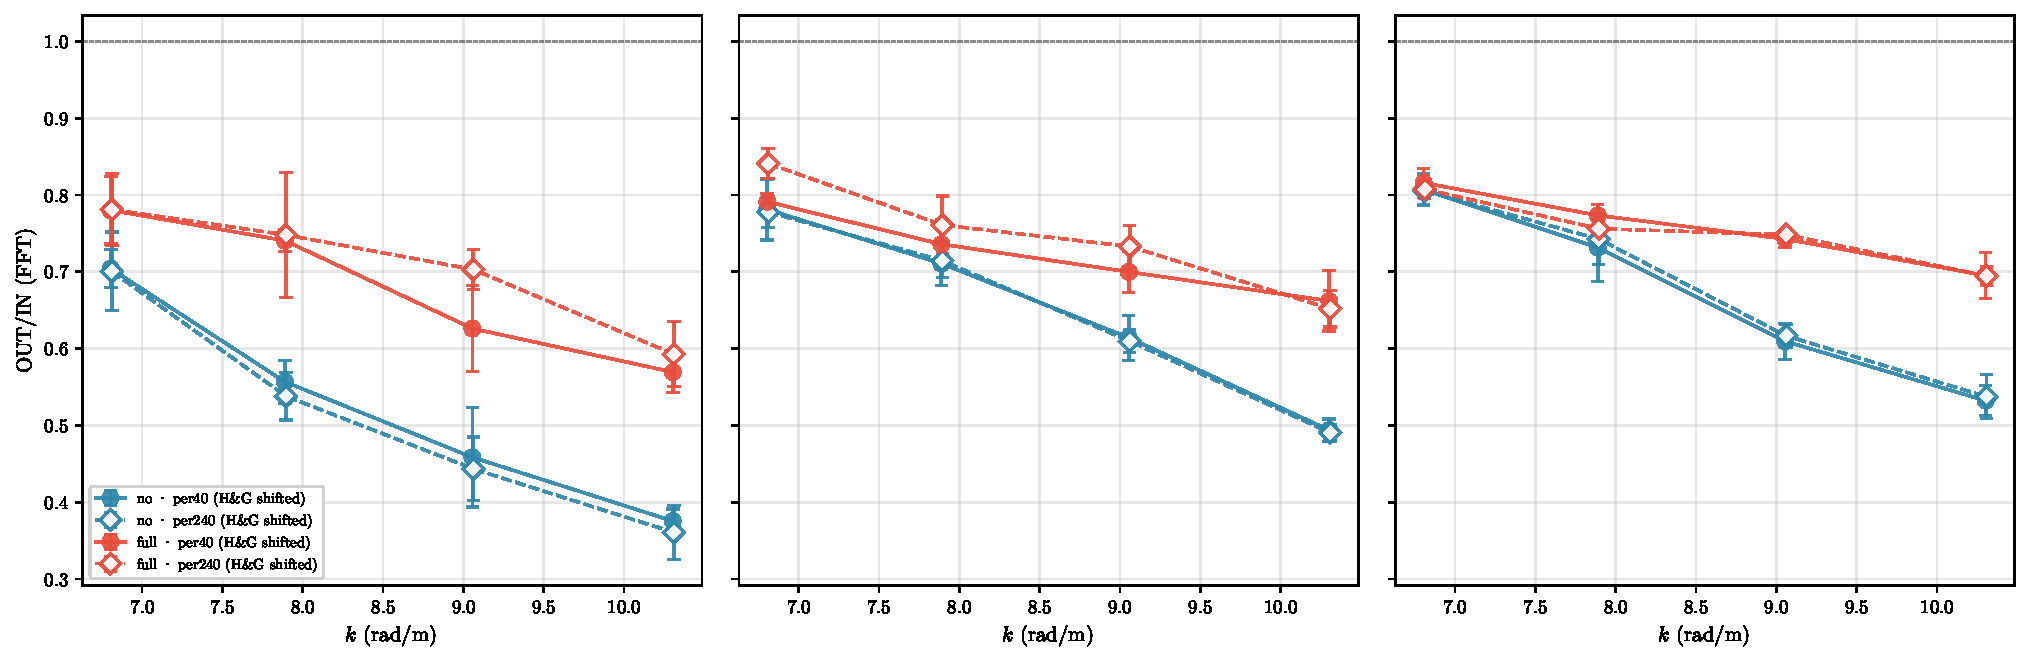
\includegraphics[width=\linewidth]{FIGURES/ch04_per40_and_per240_HG_shifted.pdf}
  \caption{
    OUT/IN (FFT) at the paddle frequency versus $k$ (rad/m), split by paddle drive 0.10, 0.20, 0.30\,V (one panel each). Both per40 (filled circles) and per240 (open diamonds) runs use the Huseby--Grue window anchored at $r = 12.4$\,m with $[50T, 60T]$ from wavemaker start. The IN probes at $r = 9.373$\,m receive the same waves $\Delta T$ earlier by group velocity ($c_g = g/(4\pi f)$, deep water), so the IN window is shifted back by $\Delta T \in [9.93, 6.55]$\,T across the thesis band. Canonical IN amplitude = mean AFFT across 9373/170 and 9373/340; OUT amplitude = AFFT at 12400/250. Blue: no wind; red: full wind. Error bars: run-to-run standard deviation. Mooring below\_90\_loose (230+300 merged), quality\_flag = ok, full panel.
  }
  \label{fig:ch04_per40_and_per240_HG_shifted}
\end{figure}
